\chapter{Technical Background}
\label{chap:chapterthree}

The architecture of IC is quite different to other blockchains. Their goal for “Blockchain singularity” comes with a lot of 
requirements. For example, the end users using the ecosystem should have their personal data more secure while having the same 
experience interacting with it as they do in a traditional IT environment.  In order to understand their architecture, we have to 
look at how they structure their infrastructure and also realise their ecosystem terminology. 

We begin this chapter by giving an overview of the IC and explaining the notion of replicated state machines. Then, we explain the 
role of 'Nodes' within the IC network, with a special emphasis on the 'Boundary node', which is used by the end users to interact 
with the IC. Following this, the concept of 'Subnets' is discussed. To achieve fault tolerance, the state machine may be replicated. 
We also highlight the difference between 'System Subnets' and 'Application Subnets', and their respective roles in IC's functionality.

Next, we delve into 'Replicas' and 'Canisters', critical components that facilitate the execution of smart contracts and distributed 
computing in the IC network. 

IC is a DAO-controlled network and roughly works as follows: each subnet runs a permissioned consensus protocol, but a decentralized 
autonomous organization (DAO) determines which entities provide replicas, configures the topology of the network, provides a 
public-key infrastructure, and controls which version of the protocol is deployed to the replicas. Hence, we dive deeper into the 
examination of the 'Consensus algorithm' used by IC. Subsequently, we delve into the 'Network Nervous System' (NNS), the DAO that 
governs the Internet Computer. A detailed understanding of NNS, its structure, and its functioning is essential in grasping how IC 
operates on a higher level.

Finally, we explore 'IC-OS', the operating system used by IC. We dissect its multiple components, including 'guestOS', 'hostOS', 
'boundary-guestOS', and 'setupOS', each playing a unique role in the operation of the Internet Computer.

This chapter sets the stage for subsequent sections by providing the necessary background information on IC technology, facilitating 
a deeper understanding of the blockchain's capabilities, strengths, and weaknesses.


\section{Nodes}

\subsection{Replica nodes}

  \textbf{The replica nodes} make up the subnet. Each replica node holds all of the states of the canisters and processes, as well as all the messages that should be processed by the canisters. The Internet Computer provides that even if some of the replicas powering the subnets are offline or even malicious, the subnet continues to process messages for the canisters. More precisely, as long as less than a third of those replicas are offline or malicious (i.e., more than two-thirds of them are online, available, and participating in the protocol), then the subnets continue making progress for replication. The network uses a consensus protocol, such that all of the replicas process the same messages via a blockchain.

\subsection{Boundary node}

  \textbf{The boundary nodes} are the gateway to the Internet Computer (IC), which allow users to seamlessly access the canister smart contracts running on it: through stock browsers users are served web-content fully from the chain. To this end, the boundary nodes translate the users' requests into API canister calls, route these calls to the subnet running the canister, and load balance among the subnet's replica nodes. In addition, boundary nodes provide caching and other services for improved performance.



\section{Subnets}

A so-called subnet is a collection of replicas that run a separate instance of the consensus mechanism to create their own blockchain on which a set of canisters can run. Each subnet can communicate with other subnets and is controlled by the root subnet, which uses chain key cryptography to delegate its authority to the various subnets.




\begin{figure}
	\begin{subfigure}[t]{.5\linewidth}
		\centering
		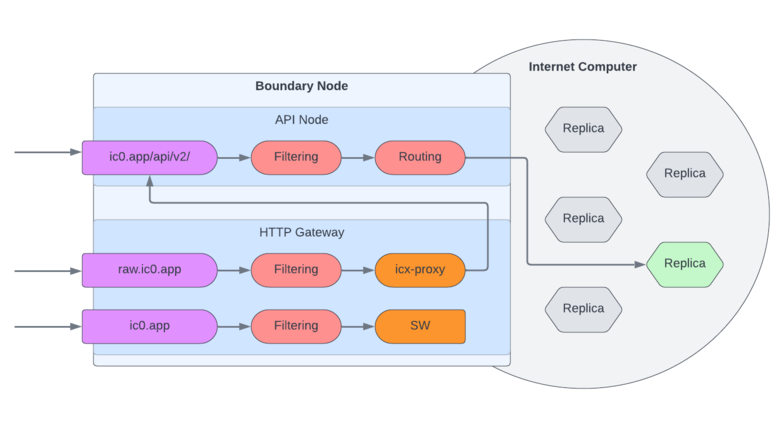
\includegraphics[width=.8\linewidth]{figures/boundary-nodes.png}
		\caption{Boundary nodes}
		\label{sfig:boundarynodes}
	\end{subfigure}
	\begin{subfigure}[t]{.5\linewidth}
		\centering
		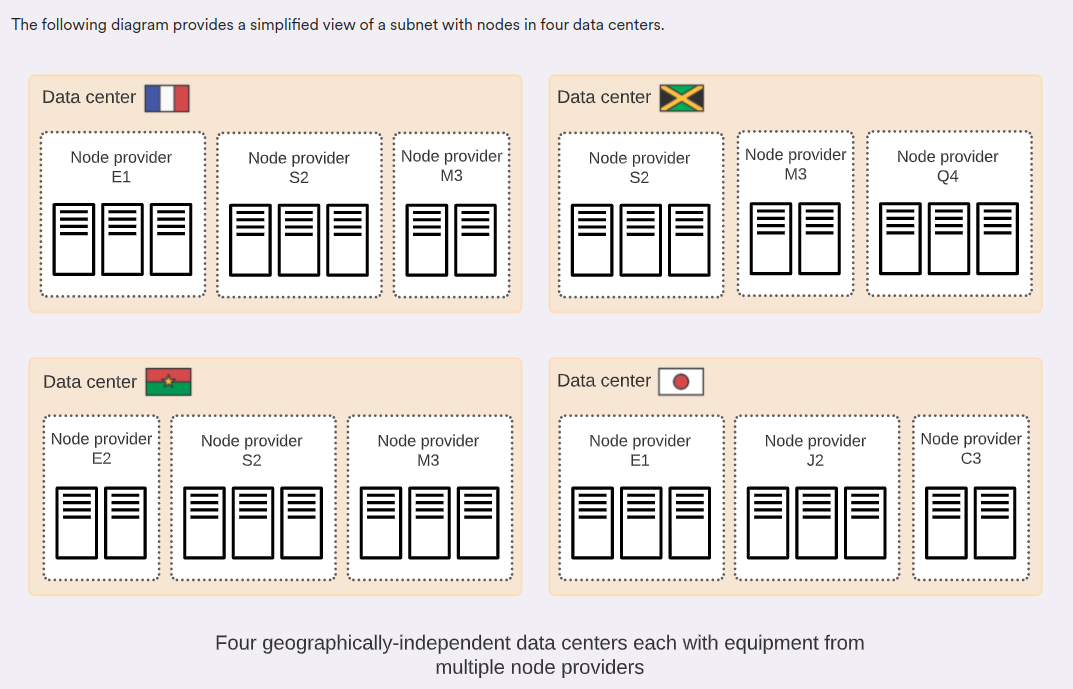
\includegraphics[width=.8\linewidth]{figures/subnet.png}
		\caption{Subnets}
		\label{sfig:subnet}
	\end{subfigure}
	\caption{Boundary nodes and subnets}
	\label{fig:icboundarysubnet}
\end{figure}

\subsection{System Subnets}

\begin{itemize}
  \item \texttt{system} subnets: These subnets are reserved for canisters that are an integral part of the Internet Computer. Typically, canisters on these subnets are controlled by the NNS and they don't pay cycles. Users cannot deploy canisters on those subnets.
\end{itemize}

\subsection{Application Subnets}

\begin{itemize}
  \item These are the default subnets that users can deploy canisters to. They typically have a size of 13 nodes, and canisters on them have to pay cycles. If a user does not provide any specific requirements, a random application subnet is chosen as the destination to create the canister.
\end{itemize}

\section{Replicas}

There can be horizontal scaling due to the introduction of subnets. Each subnet contains multiple replica sets. The core components of a replica are organized into the following logical layers:

\begin{enumerate}
  \item A peer-to-peer (P2P) networking layer that collects and advertises messages from users, from other nodes in its subnet blockchain, and from other subnet blockchains. Messages received by the peer-to-peer layer are replicated to all of the nodes in the subnet to ensure security, reliability, and resiliency.
  \item A consensus layer that selects and sequences messages received from users and from different subnets to create blockchain blocks that can be notarized and finalized by Byzantine Fault Tolerant Consensus, forming the evolving blockchain. These finalized blocks are delivered to the message routing layer.
  \item A message routing layer that routes user- and system-generated messages between subnets, manages the input and output queues for dapps, and schedules messages for execution.
  \item An execution environment that calculates the deterministic computation involved in executing a smart contract by processing the messages it receives from the message routing layer.
\end{enumerate}

\section{Canisters}

When you write source code for a dapp that runs on the Internet Computer, you compile the source code into a WebAssembly module. When you deploy the WebAssembly module that contains your program on the Internet Computer blockchain, the program is executed inside a conceptual computational unit called a canister, or canister in short. Canisters can be developed in various programming languages. Besides Motoko, a programming language purposefully designed for the Internet Computer, you can also use existing programming languages like C, Rust, JavaScript/TypeScript, AssemblyScript, and Python.

There are only two types of calls:

\begin{enumerate}
  \item non-committing \textbf{query calls} (any state change is discarded) and
  \item committing \textbf{update calls} (state changes are persisted).
\end{enumerate}

\section{DFX}

\begin{figure}
	\centering
	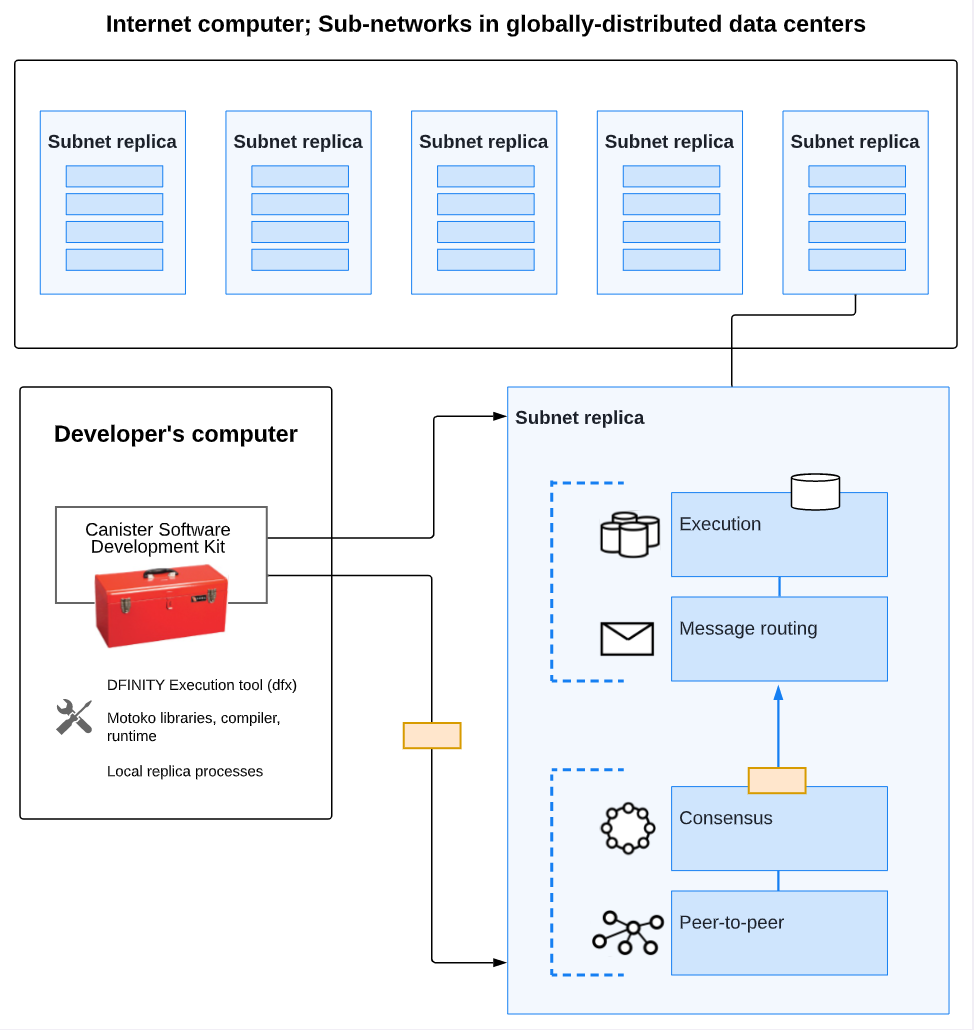
\includegraphics[width=.5\linewidth]{figures/dfx.png}
	\caption{dfx architecture}
	\label{fig:dfx}
\end{figure}


\section{Consensus algorithm}

IC is formed by a sovereign network of standardized ``node machine'' hardware operated by independent parties. To participate, nodes 
must produce the same number of blocks as others in their cohort without deviation. In a scheme of Proof-of-Useful-Work (PoUW), 
replicated smart contract computation is their work, driving optimal efficiency. Nodes form into subnet blockchains and then into a 
unified limitler, when we moved to the neess blockchain, using game-changing Chain Key Crypto.

\href{https://wiki.internetcomputer.org/wiki/Proof_of_Useful_Work}{More info about their consensus algorithm.}

Proof-of-useful-work (PoUW) involves a blockchain being produced by dedicated hardware called ``node machines'' that are of very 
similar, standardized specifications. These run highly sophisticated consensus protocols that lean into the power of advanced 
cryptography, often referred to as Chain Key Crypto. PoUW is concerned with membership in the network.

Naturally, as per PoW, the purchase, hosting and operation of node machine hardware acts as the stake. However, these machines don't 
do hashing, and simply produce and process blocks of transactions that represent smart contract computations. The reason that 
combined node machines must be built to the same standardized specification is that rather than compete to perform hashing, they must 
try not to ``statistically deviate'' by producing more or less blocks. In essence, rather than trying to perform more computation, 
they try to perform the same amount of computation and can be punished for deviating from the group.

\section{NNS - network nervous system}

A key ingredient of the scheme is the \href{https://wiki.internetcomputer.org/wiki/Network_Nervous_System}{Network Nervous System} (or NNS), a sophisticated permissionless DAO that is integrated with the Internet Computer's protocols. This fully controls the network, configuring it, and upgrading the software run by node machines. Among its responsibilities, it combines node machines to create ``subnet blockchains,'' which themselves are combined into a single blockchain using Chain Key Crypto.

This achieves two important things.

\begin{enumerate}
  \item Firstly, expense aside, it is not possible for an adversary simply to add nodes to a subnet blockchain, since the NNS carefully selects nodes by looking at the node provider, the data center the node is installed within, and its geography and jurisdiction, in a scheme of ``deterministic decentralization.''
  \item SecondlyGuestOS refers to the operating system running inside a QEMU virtual machine on the hostOS. A GuestOS image consists of the base Ubuntu system, along with the replica and orchestrator binaries. The IC protocol runs inside the GuestOS virtual machine., the NNS can remove (or ``slash'') nodes that statistically deviate.
\end{enumerate}

By applying \textbf{deterministic decentralization}, the NNS creates a highly secure scheme in which the Internet Computer runs on a sovereign network of dedicated hardware formed from node machines, which machinery can be tightly held to correct behavior in order to continue its participation in block production (through which its owners, the node providers, earn rewards). In PoUW, the repetitive hashing work of PoW, whose purpose relates primarily to network operation, has been replaced by useful smart contract computation. Since this is work that must be performed anyway, a supremely efficient network is produced.

\subsection{What is it built of?}

The Network Nervous System of the Internet Computer is realized by a set of \textit{canisters}. NNS canisters include:

\begin{enumerate}
  \item \textbf{Ledger canister}: The ledger canister stores the ICP utility \textit{token balance} of each principal and the history of ICP \textit{transactions}.
  \item \textbf{Governance canister}: The governance canister receives and stores \textit{Proposals}, which are suggestions for how the Internet Computer should be changed. These proposals can then be voted on. The governance canister also tracks \textit{Neurons}, which determine who is allowed to participate in governance.
  \item \textbf{Registry canister}: The registry canister stores the configuration of the whole Internet Computer, e.g., which nodes belong to a certain subnet and the software each node should run.
  \item \textbf{Cycles minting canister}: This canister is responsible for minting \textit{cycles}, the fuel for canisters for computation, communication, and storage. New cycles can be minted when a new canister is newly created or when an existing canister is topped up with additional cycles.
  \item \textbf{Root canister}: The root canister is the controller of all other NNS canisters and responsible for upgrading them.
  \item \textbf{Lifeline canister}: The lifeline canister is the controller of the root canister and responsible for upgrading it.
  \item \textbf{Archive canisters}: The canisters that store the history of the ledger transactions once there are too many transactions to keep in a single canister.
  \item \textbf{Genesis token canister}: This is the canister that was used to initialize the neurons that already existed during genesis.
\end{enumerate}

The canisters that users of the Internet Computer are interacting with the most are the first two: the ledger canister for making transactions, and the governance canister for staking tokens and submitting and voting on proposals.



\section{IC-OS}

IC-OS contains:

\begin{itemize}
  \item \textbf{SetupOS:} Responsible for booting a new replica node and installing HostOS and GuestOS.
  \item \textbf{HostOS:} The operating system that runs on the host machine. Its main responsibility is to launch and run the GuestOS in a virtual machine. In terms of its capabilities, it is intentionally limited by design.
  \item \textbf{GuestOS:} The operating system that runs inside a virtual machine on the HostOS. The core IC protocol is executed within the GuestOS.
  \item \textbf{Boundary-guestOS:} The operating system that runs on boundary nodes.
\end{itemize}

The Ubuntu-based IC OS is built by:

\begin{itemize}
  \item Creating a root filesystem image using docker -- this is based on the official Ubuntu docker image and simply adds the OS kernel plus our required services to it.
  \item Converting this root filesystem into filesystem images for +/+ and +/boot+ via +mke2fs+.
\end{itemize}

\textbf{Docker Image:}

There are two dockerfiles for each of the OS

1. \textbf{Dockerfile.base}

The Dockerfile.base takes care of installing all upstream Ubuntu packages because the versions of these packages can change at any given time.

In order to maintain build determinism, once a week, the CI pipeline builds a new base image for each OS.

2. \textbf{Dockerfile}

The Dockerfile builds off the published base image and configures and assembles the main disk-image.

The docker image is then transformed into a bootable "bare-metal" or "virtual-metal" VM image for use outside containerization.

\subsection{guestOS}
GuestOS refers to the operating system running inside a QEMU virtual machine on the hostOS. A GuestOS image consists of the base Ubuntu system, along with the replica and orchestrator binaries. The IC protocol runs inside the GuestOS virtual machine.

\subsection{hostOS}

The term HostOS is used for the operating system running on the physical machine. The purpose of this system is to enable virtualization for any node running on top.

\subsection{boundary-guestOS}

\subsection{setupOS}

SetupOS is used for the operating system installing the IC-OS stack.

The sequence of the scripts is defined in the main installation script, \texttt{setupos.sh}. The order of execution is as follows:

\begin{itemize}
  \item \texttt{hardware.sh}: Verifies the system's hardware components.
  \item \texttt{network.sh}: Tests network connectivity and reachability of the NNS.
  \item \texttt{disk.sh}: Purges existing LVM configurations and partitions.
  \item \texttt{hostos.sh}: Installs and configures the HostOS operating system.
  \item \texttt{guestos.sh}: Installs and configures the GuestOS operating system.
  \item \texttt{devices.sh}: Handles the HSM.
\end{itemize}
